%Document Class - Article

\documentclass[14pt]{report}

%Preamble

\title{Comprehensive Guide to Zoom}
\author{By Jerry Akshay, the Tech Head}

\usepackage{indentfirst}
\usepackage{array}
\usepackage[utf8]{inputenc}
\usepackage{graphicx}
\usepackage{geometry}
\usepackage{extsizes}
\usepackage{fancyhdr}
\usepackage{titleref}
\usepackage{tabularx}
\usepackage{lmodern} % for bold teletype font
\usepackage{amsmath}  % for \hookrightarrow
\usepackage{xcolor}   % for \textcolor
\usepackage{listings}
\usepackage{subfig}
\usepackage{float}
\lstset{
  basicstyle=\ttfamily,
  columns=fullflexible,
  frame=single,
  breaklines=true,
  postbreak=\mbox{\textcolor{red}{$\hookrightarrow$}\space},
}
\graphicspath{ {./images/} }
\usepackage [english]{babel}
\usepackage [autostyle, english = american]{csquotes}
\MakeOuterQuote{"}

\newcommand{\changefont}{
    \fontsize{10}{10}\selectfont
}

%Page Margins and Dimensions
\geometry{		
	a4paper,
	total={170mm,257mm},
	left=25mm,
	top=25mm,
	right=25mm,
	bottom=25mm,
	}

%Header
\pagestyle{fancy}
\fancyhf{}
\rhead{Comprehensive Guide to Zoom}

\renewcommand{\contentsname}{Table of Contents}

\renewcommand{\headrulewidth}{2pt}
\renewcommand{\footrulewidth}{0.4pt}



\begin{document} %Document Begins

	%Title Page

 	\maketitle
	\pagenumbering{gobble} %Disable Page Numbering

	\newpage

	%Acknowledgement

	\chapter*{Preface}\label{chapter}
		
		\lhead{\titleref{chapter}}

        So, you're stuck in this lockdown amidst the COVID-19 pandemic. These surely are unsure times (The irony is strong with this statement). But, does that mean that you can't meet or see the group of people you used to hang out with? Absolutely fudging not!\\
        
        There is an app called `Zoom Cloud Meetings' that can help you meet the same set of people virtually, as long as you have a working internet connection.\\

        Know nothing about this app? Don't worry. That's why I exist right? To clear all your doubts - be it stupid, unforgiving or perfectly valid - use this comprehensive guide to guide you through the process of installing and using `Zoom' the right way.\\

        Still think it's too good to be true? Well then, you just might be pleasantly surprised. Just check out the rest of document. You might need to schedule an appointment with the doctor though - because your jaw would drop.\\

        Still be cautious of COVID-19 though. Pray that it doesn't spread much further. Speaking of that, spread this document across like COVID-19. (For legal reasons, that's a joke.)

    \newpage

    \lhead{Table of Contents}

	\renewcommand{\footrulewidth}{0pt}

	\tableofcontents

    \newpage
    
    \listoffigures

    \newpage

    \renewcommand{\footrulewidth}{0.4pt}

	\pagenumbering{arabic} %Use Page Numbering from here


	%Footer
    \fancyfoot[R]{\changefont Page \thepage}
    
    \fancypagestyle{plain}{%
		\fancyhf{}%
		\fancyfoot[R]{Page \thepage}%
		\renewcommand{\headrulewidth}{0pt}% Line at the header invisible
		\renewcommand{\footrulewidth}{0.4pt}% Line at the footer visible
		}
    
    \chapter{Introduction}\label{chapter1}
		
        \lhead{\titleref{chapter1}}

        \section{What is the `Zoom Cloud Meeting' App?}
            The `Zoom Cloud Meeting' App is an application that enables you to virtually host or join meetings (Now you can't really escape those boring ass office meetings).\\

            In simpler terms, it basically enables you to be a part of conference calls. It enables the participants of the conference call to join the call via audio (mic), video (camera), and also provides the ability to share the screen (Be mindful of what's on your screen though - better safe than sorry).\\

        \section{Applications of this App}
            The Zoom App can be used for the following purposes:
            \begin{itemize}
                \item Virtual Office Meetings
                \item Virtual Prayer Meetups 
                \item Virtual Masses
                \item Virtual Boss Screwing Sessions
                \item Virtual Drug/Alcohol Addict Interventions
                \item Virtual Classes
                \item Virtual Piracy of Movies
                \item Virtual One-on-One Meetups (aka Dates)
                \item The only way to meet up with an unhygienic person
            \end{itemize}

        \section{Who made this wonderful piece of software?}
            Definitely not me, that's for sure. You gotta thank the folks over at `Zoom Cooperation' for that. Although, the workload on their servers currently are definitely spiked up due to the lockdown. Either they made the best or the worst decision of their lives making this piece of software.   
        
    \newpage

    

	%Project Snapshots

	\chapter{Installation}\label{chapter2}
		
	\lhead{\titleref{chapter2}}
            \section{How do you install this piece of jewel?}
                It's very simple. All you need is a phone with an app store. This phone can either be the poor man's Android or the rich man's iPhone. If you have a Windows phone, the whole world mourns your loss.\\

                Now, you have the above mentioned pieces of technology. What should you do now? Well, follow the rest of the guide in order. It probably might bring the long lost peace in your life, or might be horribly and horrifically ruin your life. Either way, I'm still gonna be guiding you. Yaaay me!

                \subsection{Access the App Store to search for the App}
                    If you expected a different title, I'm sorry. I can only be as much straightforward as this. Now, coming to the matter at hand, search for `Zoom Cloud Meetings' on the App Store and click on `Install Application' button.\\

                    I'm pretty sure by now you would know how to access the App Stores on your phone. If you don't, then you might be using the wrong guide... or quite possibly on the wrong planet.\\

                    If you've done the above steps correctly, you just need to wait for the app to complete it's installation. Patience is key during times like this. Probably count the number of times TV9 keeps showcasing divorce cases on TV. It'll keep you going.\\

                    Once the app has been installed, you're good to proceed to the subsequent steps.\\
                    \begin{figure}[H]
						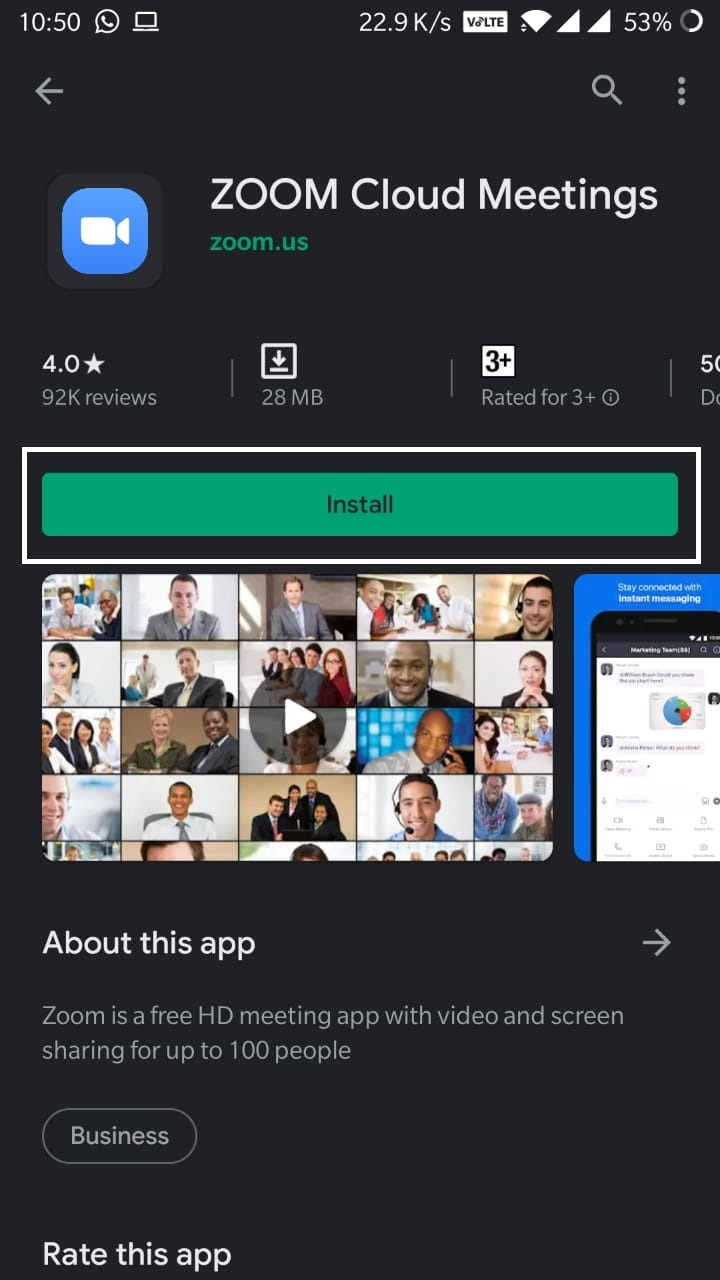
\includegraphics[width=6cm]{ZoomApp.jpeg}
						\centering
                        \caption{Zoom App on the Play Store}
                        \label{fig:ZoomApp}
					\end{figure}

                    Figure~\ref{fig:ZoomApp} depicts the App as is seen on the Play Store. (Yes, I'm a poor nibba with an Android phone)
                    
    \newpage
    
    \chapter{Application Usage}\label{chapter3}
		
    \lhead{\titleref{chapter3}}

    \section{How do you open the app?}
                    If you're reading this part, you most definitely don't deserve a phone. But, since you reached this part, I'm gonna help you nonetheless.\\

                    All you have to do is open your phone's App drawer and scroll through the endless list of all the useful/useless apps you might have to find this jewel - Zoom.\\
                    \begin{figure}[H]
						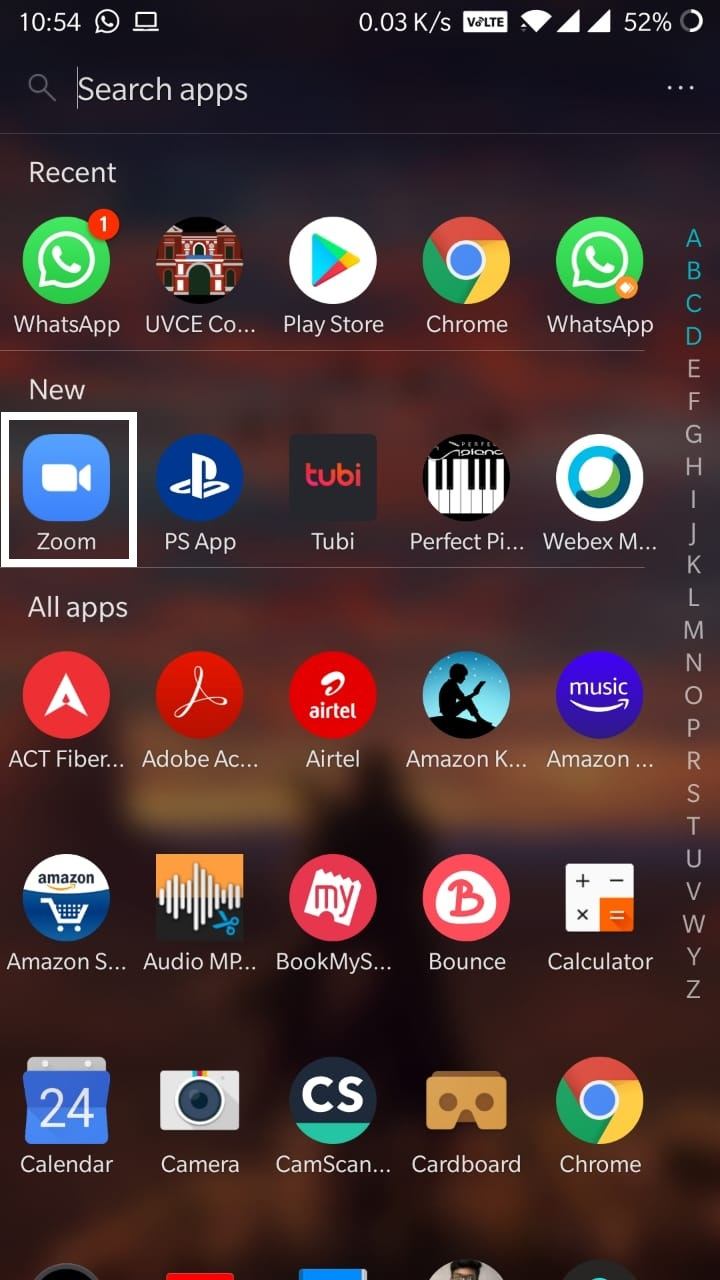
\includegraphics[width=6cm]{ZoomAppDrawer.jpeg}
						\centering
                        \caption{Zoom App in your App Drawer}
                        \label{fig:ZoomAppDrawer}
                    \end{figure}
                    
                    Once you've found this jewel, tap on it to open it (or howl at your phone - don't blame me if this doesn't work).
    \section{What do you do once you have opened this forbidden treasure?}
                    Once you have opened the app, you'll be presented with the following set of annoying pages. What you choose to do can either make or break your phone. So, be wary and cautious in your approach.\\

                    Rest assured, if you follow the steps in the order I show, you have nothing to worry about. You probably might have a spot saved in heaven for all I know.\\

                    \subsection{First Time Use Page}
                        This page is the page you see once you open the app for the first time. Here, you'll be presented with three options:
                        \begin{figure}[H]
                            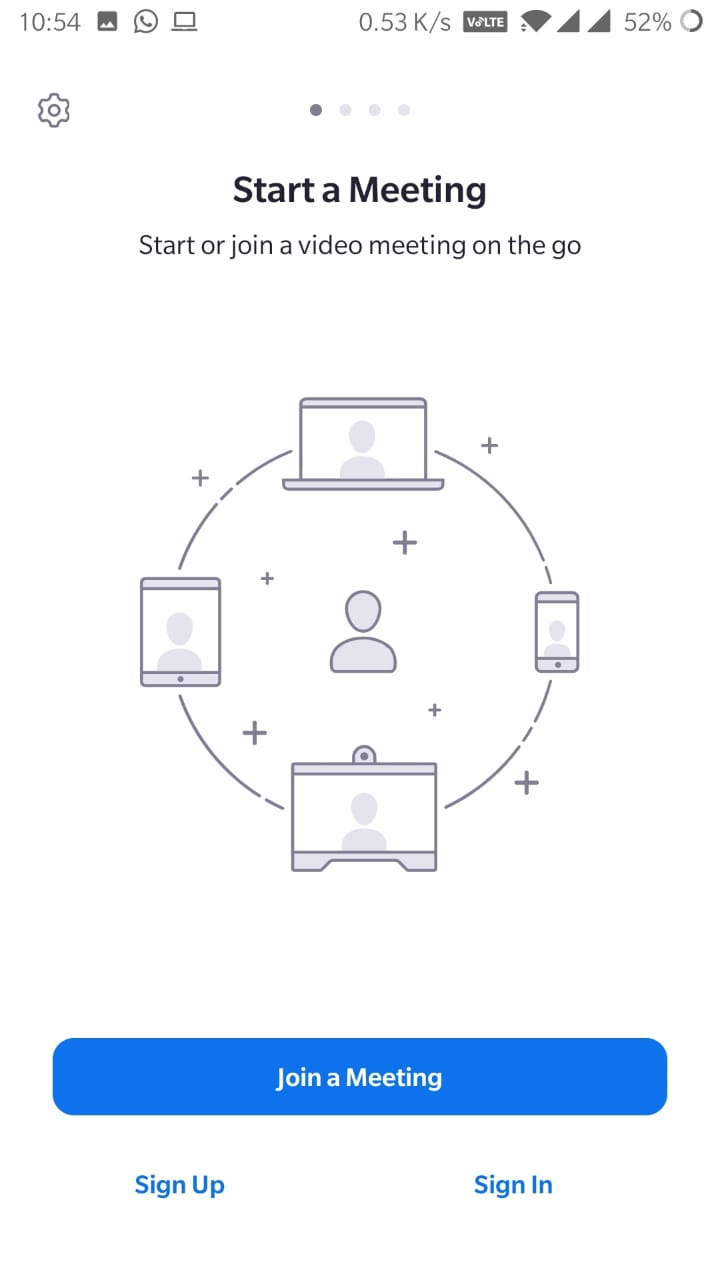
\includegraphics[width=6cm]{LandPage.jpeg}
                            \centering
                            \caption{First Time Use Page}
                            \label{fig:LandPage}
                        \end{figure}
                        \begin{enumerate}
                            \item Join a Meeting
                            \item Sign Up
                            \item Sign In
                        \end{enumerate}

                        Well, since you might want to use the App on a regular basis during the lockdown, I suggest you choose the `Sign Up' or the `Sign In' option. Only if you're a sad loner should you choose the `Join a Meeting' option.\\

                        The `Sign Up' option will allow you to create a new Zoom account. The `Sign In' option will allow you to log in (or sign in) to an already existing Zoom account. You can also use the `Sign In' option to create an account and login to the app via Google Sign-in or Facebook Sign-in. Figure~\ref{fig:SignOptions} depicts the Sign-Up / Sign-In options.\\
                        \begin{figure}[H]
                            \centering
                            \subfloat[Sign-Up Page]{{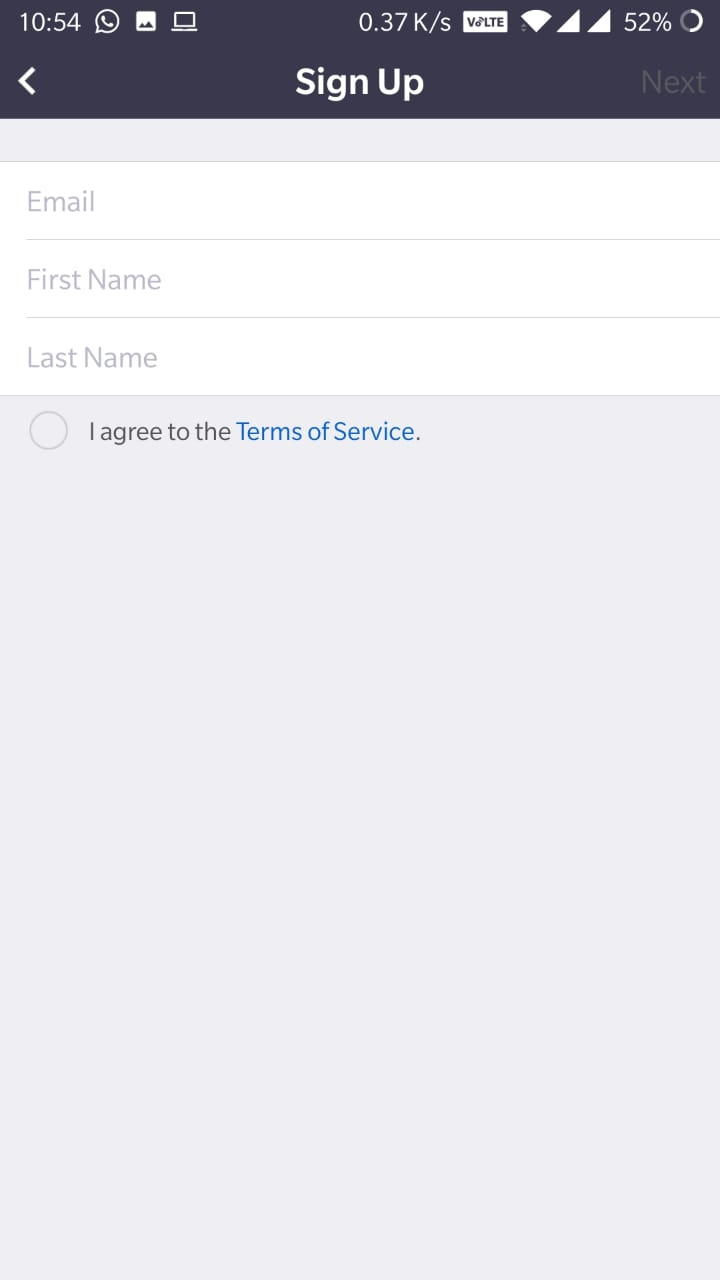
\includegraphics[width=6cm]{SignUp.jpeg} }}%
                            \qquad
                            \subfloat[Sign-In Page ]{{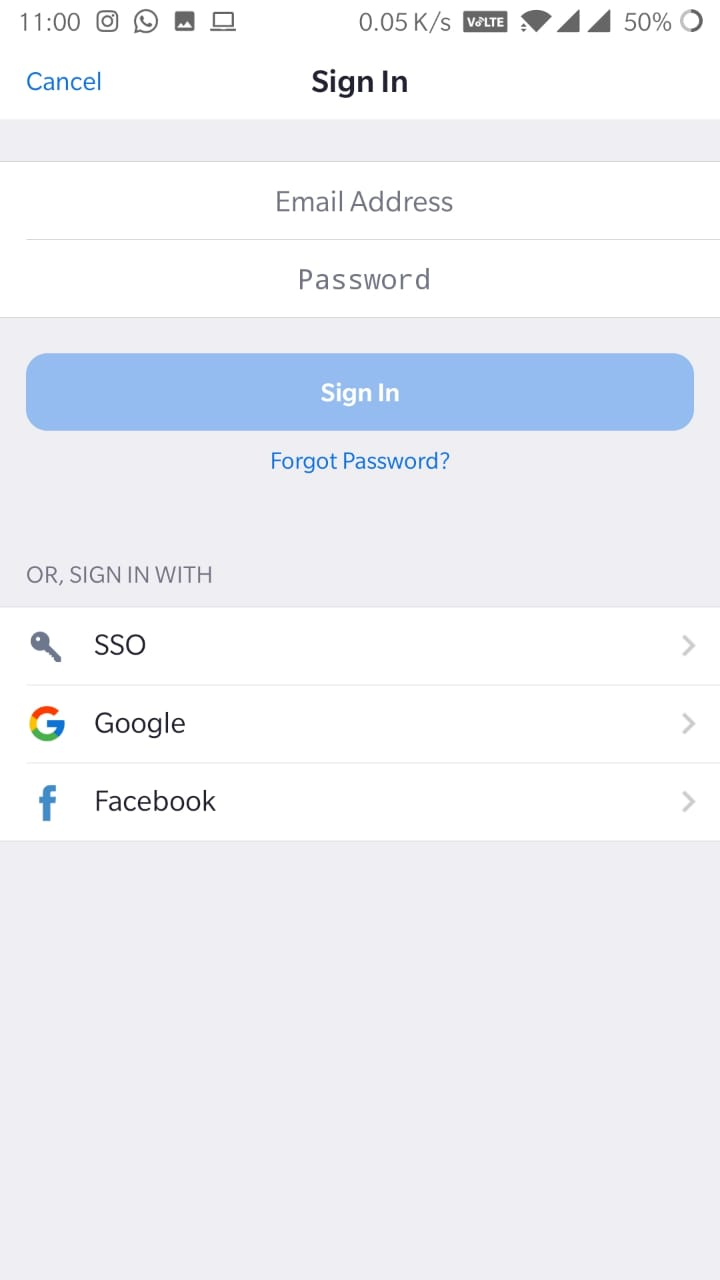
\includegraphics[width=6cm]{AlternativeSign.jpeg} }}%
                            \caption{Sign-Up / Sign-In Options}%
                            \label{fig:SignOptions}%
                        \end{figure}

                        Well, if you've successfully created an account and logged into your account, congrats! It's certainly no Mt. Everest though, but commendable nonetheless. Now, we can move forward.

                    \subsection{Landing Page}
                        The landing page is the page that shows up first whenever you subsequently open the Zoom app, provided you've created and logged into your Zoom account.\\
                        \begin{figure}[H]
                            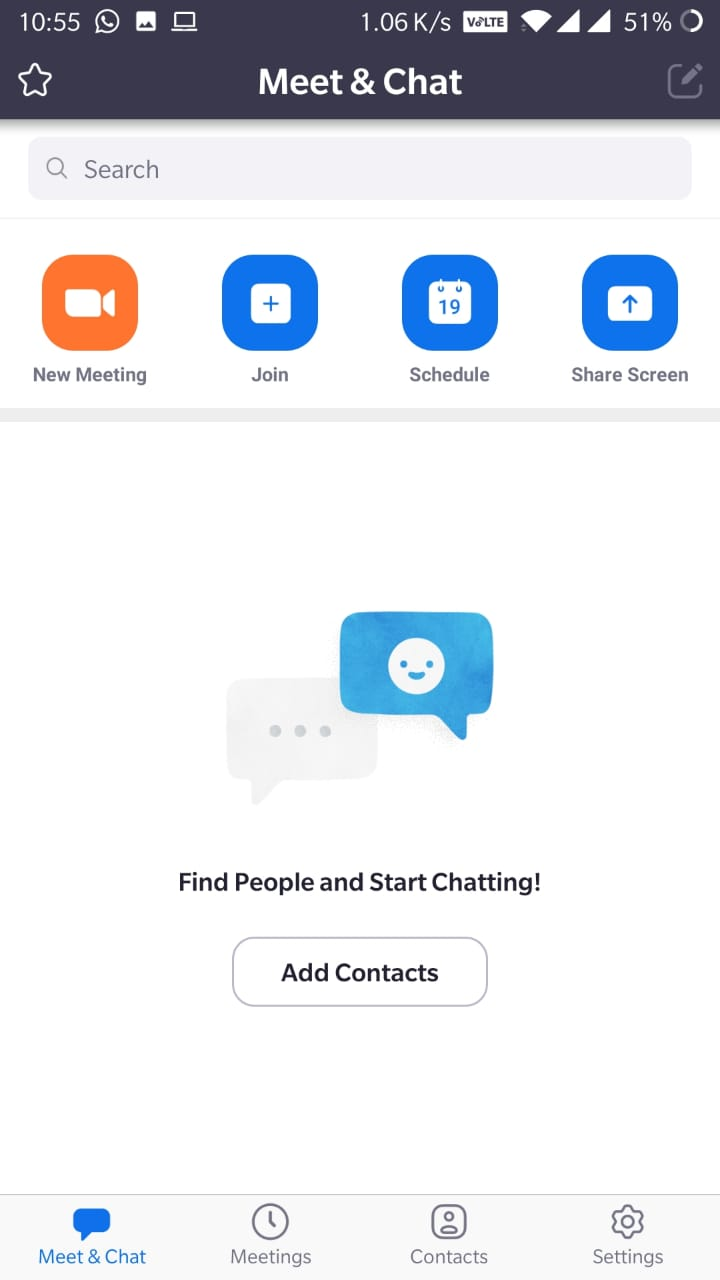
\includegraphics[width=6cm]{MainScreen.jpeg}
                            \centering
                            \caption{Landing Page}
                            \label{fig:LandingPage}
                        \end{figure}

                        The Zoom landing page provides you with a bunch of options. If you want to take the risk, experiment away. Don't blame me if your phone blows up though (or better yet, if the NSA secretly spies on you. Crap, they're onto me now.) The list of options that the Landing Page provides you in the upper half of the screen are as follows:
                        \begin{enumerate}
                            \item \textbf{New Meeting - }To start or host a new meeting of your own, where you get to be the boss. It certainly gives a feeling of power.
                            \item \textbf{Join (A Meeting, Obviously) - }Join a meeting hosted by someone else. Pretty sad, you have to act like a slave.
                            \item \textbf{Schedule (Again, a Meeting) - }If you're lazy to have a meeting now, why not have it later? This option allows you to do that. This certainly satisfies the `Lazy Man's Creed'.
                            \item \textbf{Share Screen (Please be Mindful) - }To share your screen to the nibba who's too interested in your personal matters.
                        \end{enumerate}

                        The footer of the page also provides you with a bunch of tabs. They are:
                        \begin{enumerate}
                            \item \textbf{Meet and Chat (Ahem) - }This tab basically provides the above options I discussed.
                            \item \textbf{Meetings - }This tab contains the list of scheduled and open meetings linked with your account. If you work in a company, please don't open this. You might get a heart attack.
                            \item \textbf{Contacts - }This tab allows you to find your contacts who also use Zoom, probably like that imaginary girlfriend of yours.
                            \item \textbf{Settings - }This tab allows you to change certain settings of the app such as your profile name, etc.
                        \end{enumerate}

                    \subsection{How do I join a meeting?}
                        Joining a meeting is very simple. There are 2 ways you can do this - by entering the Meeting ID directly or by tapping on the invite link sent by that one annoying friend of yours.
                        \subsubsection{Join a Meeting with the help of Meeting ID}
                            While there are people who provide you with invite links to make your job easier, there might also be some real turd who just shares the Meeting ID with you. In such cases, please use the `Join' option as seen on the Landing Page.\\

                            Figure~\ref{fig:JoinMeet} depicts the process of joining an ongoing meet with the help of a Meeting ID. Once you're in the `Join Meeting Page', you can enter the Meeting ID in the highlighted area. You even have the choice to change your display name (to either I. P. Freely, Joe Mama, etc.). If you want to, you can play around with the `Don't Connect to Audio' and the `Turn Off My Video' options. They're pretty much straightforward.\\
                            \begin{figure}[t]
                                \centering
                                \subfloat[Landing Page]{{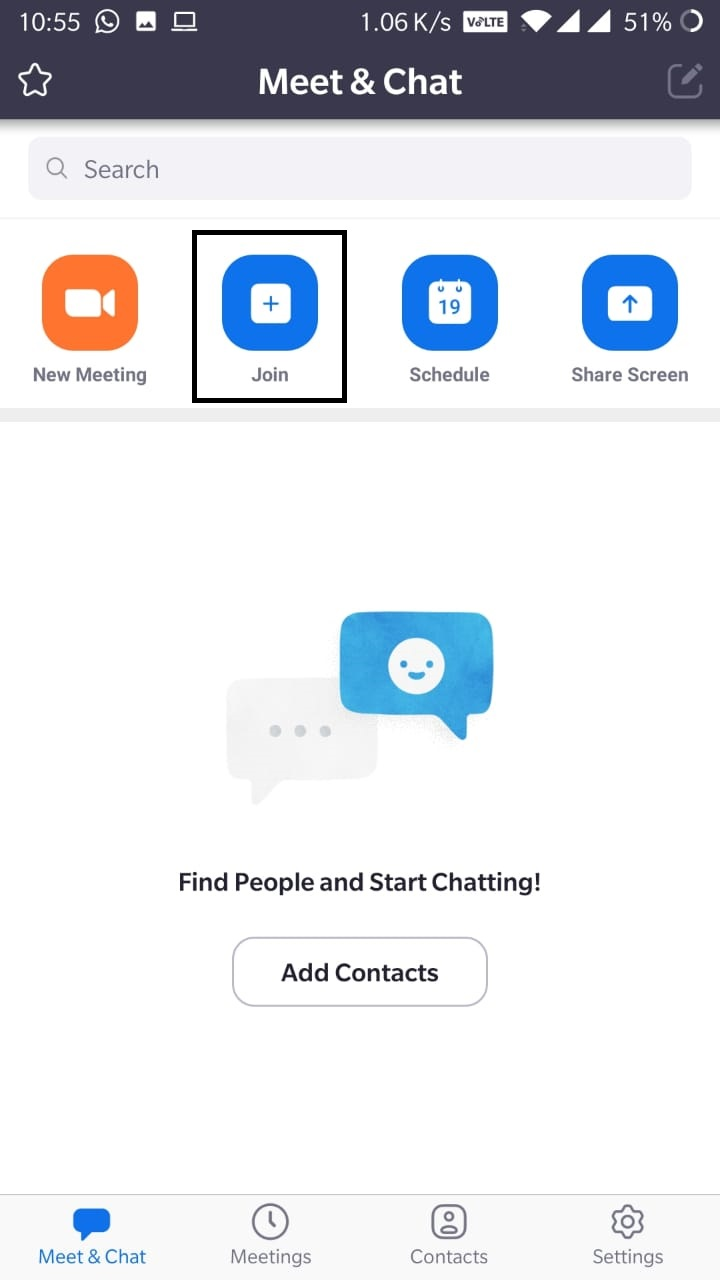
\includegraphics[width=6cm]{MainScreen1.jpeg} }}%
                                \qquad
                                \subfloat[Join Meeting Page]{{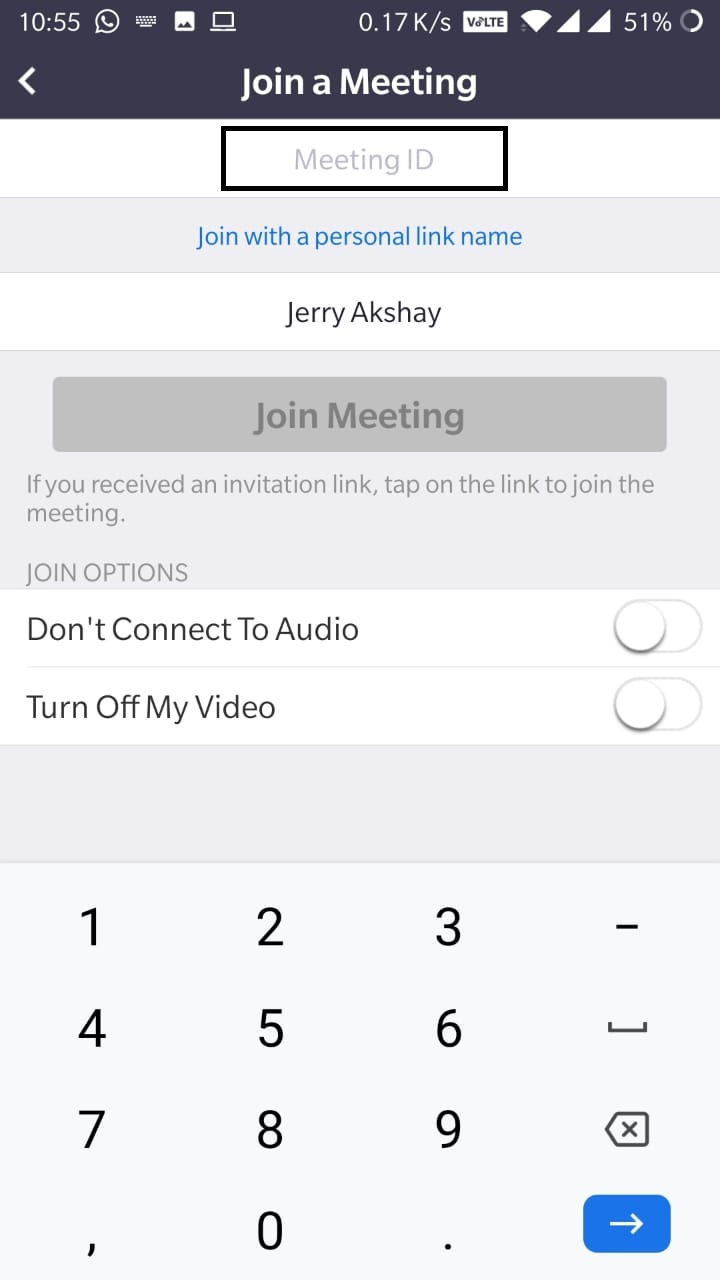
\includegraphics[width=6cm]{JoinMeet.jpeg} }}%
                                \caption{Joining a Meeting}%
                                \label{fig:JoinMeet}%
                            \end{figure}

                            Once you've followed the above steps, hit `Enter' and you'll be a part of your dream meeting! (Just kidding, it could be your worst nightmare.)

                        \subsubsection{Join a Meeting with the help of an Invite Link}
                            Now, you might have certain people in life who might be annoying, but intelligent nonetheless. These are the ones who give you a direct link. All you have to do is tap on the link and v\'oil\`a! You're part of the meeting!\\
                             \begin{figure}[h]
                                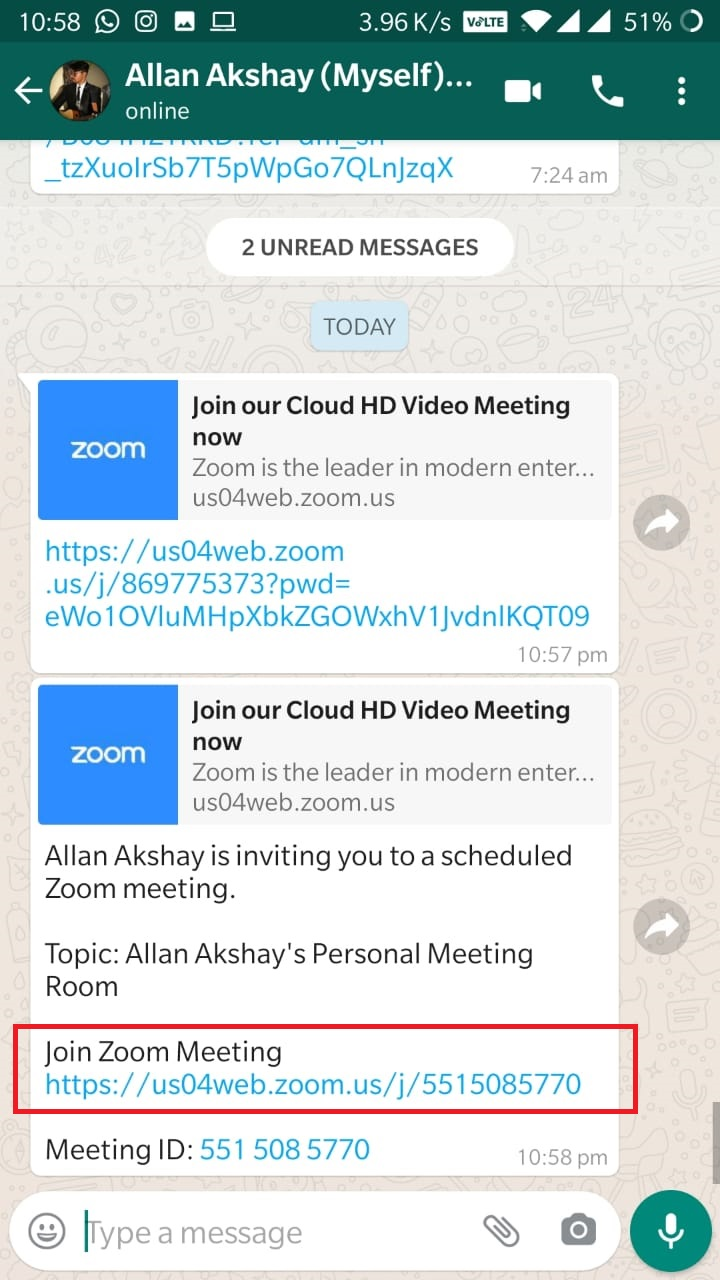
\includegraphics[width=6cm]{Invite.jpeg}
                                \centering
                                \caption{Invite Link}
                                \label{fig:InvitePage}
                            \end{figure}
                            \begin{figure}[h]
                                \centering
                                \subfloat[App Choice]{{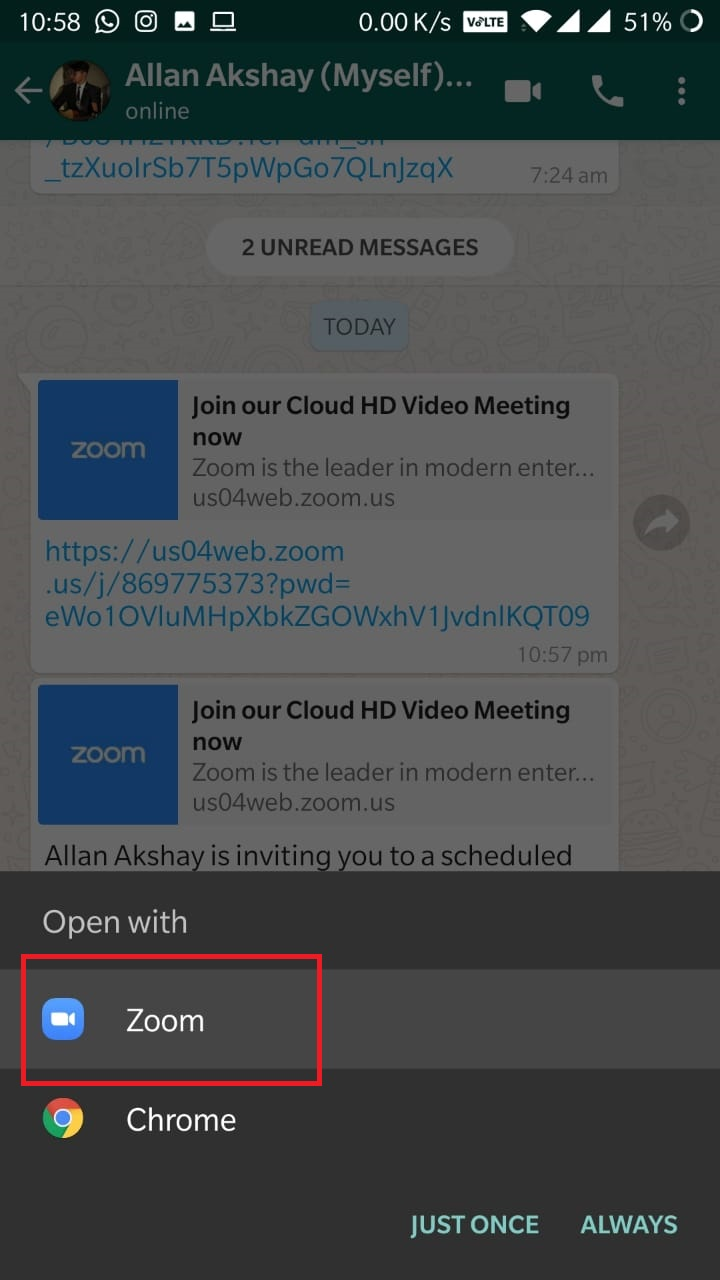
\includegraphics[width=6cm]{OpenWith.jpeg} }}%
                                \qquad
                                \subfloat[Launch Zoom]{{
\includegraphics[width=6cm]{LauchZoom.jpeg} }}%
                                \caption{Invite Link Extras}%
                                \label{fig:InviteAppPage}%
                            \end{figure}

                           

                            Figure~\ref{fig:InvitePage} depicts the meeting invite link. All you need to do is tap on that highlighted link and you're done. You're all set and into the meeting of your dreams! Quite possibly a nightmare too. Figure~\ref{fig:InviteAppPage} specifies the app to choose to join the meeting. Obviously, it has to be Zoom (unless you're feeling too lucky). Just in case you're presented with a second screen as shown in the figure, tap on the `Launch Zoom' link to jump right into the meet!


                        
                    \subsection{I've entered a meeting. What do I do now?}
                            If it's the first meeting you're attending via the App, you might have to accept a bunch of permissions. Just grant all of them and don't ask further questions. Figure~\ref{fig:PermScreen} depicts the permissions and your appropriate actions.\\
                            \begin{figure}[h]
                                \centering
                                \subfloat[Zoom Permission]{{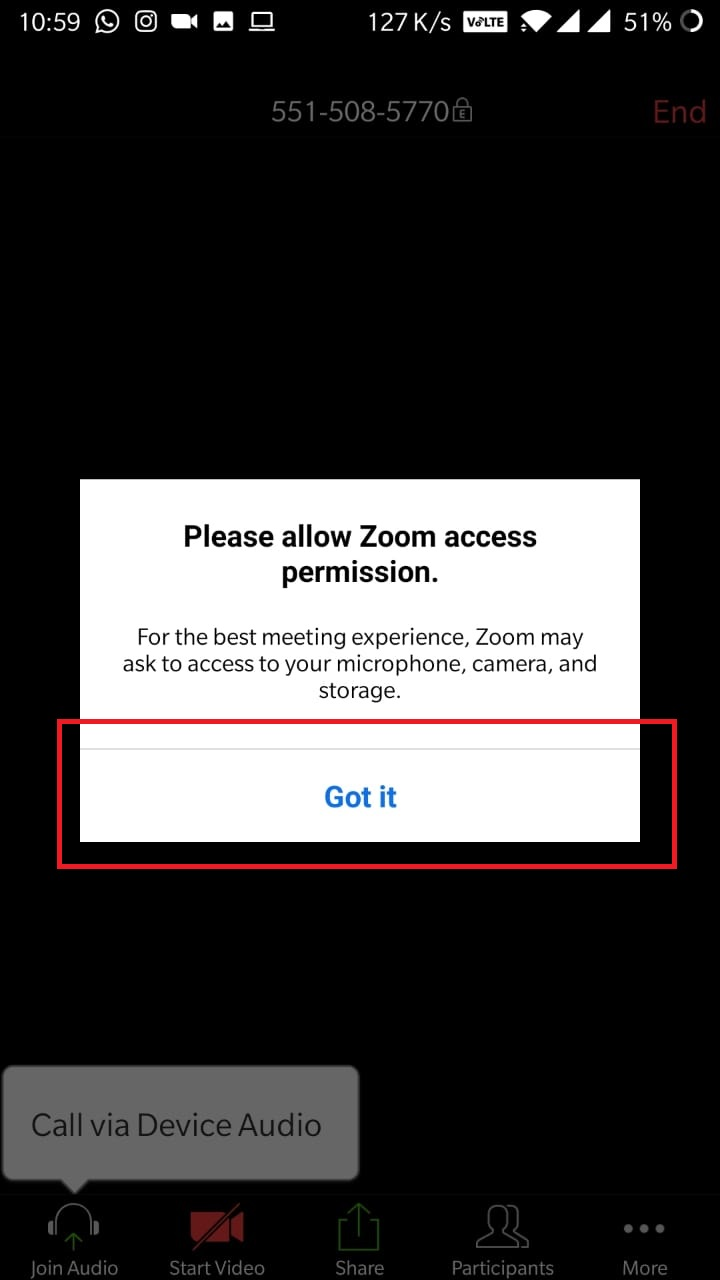
\includegraphics[width=6cm]{Perm.jpeg} }}%
                                \qquad
                                \subfloat[Audio Permission]{{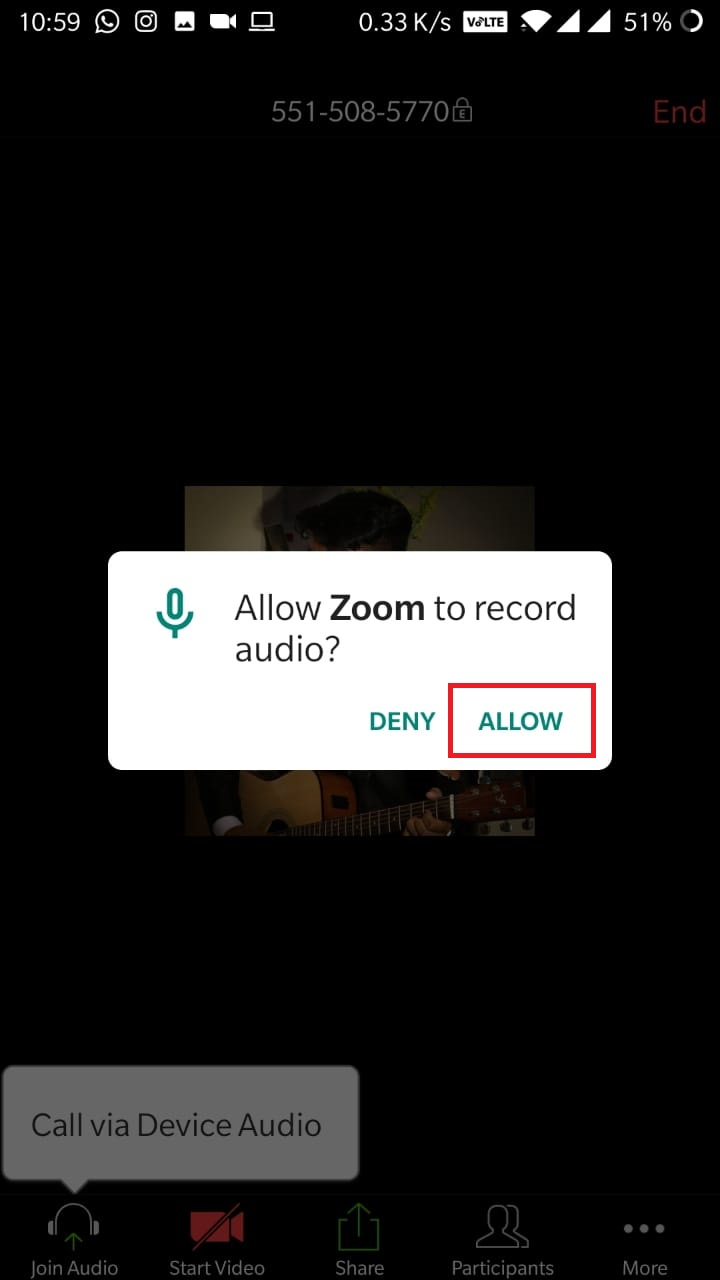
\includegraphics[width=6cm]{AudioPerm.jpeg} }}%
                                \caption{Meeting Screen Options}%
                                \label{fig:PermScreen}%
                            \end{figure}

                            Once you've entered the virtual meeting, you might encounter a lot of fumbling, noise, shouting, someone's dog barking, someone's demon being summones, just to name a few. In times like these, do not panic. These are common scenarios that can be only be wiped away by COVID-19. (Again, for legal reasons, that's a joke.)\\

                            The meeting screen enables you to join the meeting via your audio devices (mic and speaker), via video (camera), and it also enables you to share your screen. It also helps you to see all the participants of the meeting (maybe you could find your cruch attending the meet). Try exploring all the options. One key thing to keep in mind is to make sure you join the meet by Audio first. You'll have the opportunity to mute your mic later (just in case your mom comes barging into your room, screwing you for wasting time on Zoom).\\
                            \begin{figure}[h]
                                \centering
                                \subfloat[Meeting Screen]{{
\includegraphics[width=6cm]{MeetScreen.jpeg} }}%
                                \qquad
                                \subfloat[Join Meeting via Audio]{{
\includegraphics[width=6cm]{CallDevice.jpeg} }}%
                                \caption{Meeting Screen Options}%
                                \label{fig:MeetScreen}%
                            \end{figure}

                            Once you've done all this, you have successfully become part of the Zoom meeting. You have done your best by following this guide. You are a great person! Keep experimenting with the options to figure your way completely through the app.\\

                        \subsection{How do I exit the Meeting?}
                            The best part of any meeting is leaving it. As such, it's really easy to leave a meeting in Zoom. Once you're in the meeting, you just have to tap the `End' button on the upper-right portion of the screen.\\
                            \begin{figure}[h]
                                
\includegraphics[width=6cm]{EndMeet.jpeg}
                                \centering
                                \caption{Ending / Leaving a Meeting}
                                \label{fig:EndMeet}
                            \end{figure}

                            Figure~\ref{fig:EndMeet} depicts the process of ending / leaving a meeting. Just tap the button and you're away from that excuse of bandwidth!

                        \subsection{Want to host your own Meeting?}
                            Well, somebody's surely feeling like a boss today. If you really want to do this, do this in your own time and experiment with it's features. Only people who aren't afraid to venture into the dark can host their own meetings. Figure out what to do and live life happily. I'm done with my task.\\

                            There you have it! A truly comprehensive guide to Zoom that lives upto its name. No doubt whatsover!

                        
    \newpage

	%Conclusion

	\chapter*{Conclusion}\label{chapter6}
		
	\lhead{\titleref{chapter6}}
                            I hope you learnt a lot from this truly comprehensive guide. Hope it helped you conquer your fears. If in need of extra guidance and support, feel free not to contact me!
                        
	\newpage

	%References

	\chapter*{References}\label{chapter7}
		
	\lhead{\titleref{chapter7}}
                            
            \begin{itemize}
                \item Me
                \item Myself
                \item and I
            \end{itemize}

	\newpage


\end{document} %Document Ends